

\section{\tc Protocol}

We now describe the operation of \tc at the protocol level. The basic protocol is conceptually simple: A user contract \reqcont requests a datagram from the \tcontract \tcont. \tcont forwards the request to \engine and then returns the request to \reqcont. There are many details, however, relating to message contents and protection and the need to connect the off-chain parts of \tc with the blockchain.

First, we give a brief protocol overview. Then we specifying the data flows in \tc. Finally, we provide a component-level view of the protocol by specifying the functionalities embodied in the \tcontract, \medname, and \encname. We present these  as ideal functionalities, inspired by the universal-composability (UC) framework, in order to abstract away implementation details and as a springboard for formal proofs of security. We omit details in this section on how payment is incorporated into \tc; this delicate aspect of the system design is deferred to Section~\ref{}.

\subsection{Datagram lifecycle}

The lifecycle of a datagram may be briefly summarized in the following steps:

\begin{itemize}
\item {\bf Initiate request.} \reqcont sends a datagram request to \tcont on the blockchain.

\item {\bf Monitor and relay.} The \medname monitors \tcont and relays incoming datagram requests to the \encname.

\item {\bf Securely fetch feed.} Based on \dgform, the \encname contacts a data source via HTTPS and obtains the requested datagram. It forwards the datagram via the Relay to \tcont.

\item {\bf Return datagram.} \tcont checks the correctness of \dgform and returns the datagram to \reqcont.
\end{itemize}

We now make this data flow more precise. 

\subsection{Data flows}

A datagram request by \reqcont takes the form of a message $m_1 = (\dgid, \dgcallback, \dgform)$ to \tcont on the blockchain. Here, $\dgid$ is a unique request identifier (which we explain later how to compute in practice); $\dgcallback$ specifies the entry point in \reqcont to which the datagram is to be returned. (In principle, $\dgcallback$ could specify an entry point in a different contract, but \tc does not yet adopt this generalization. $\dgform$ specifies the requested datagram, e.g., ${\sf params} := (\weburl, {\sf spec}, T)$, where $\weburl$ is the target data source and {\sf spec} specifies content of a the datagram to be retrieved (e.g., a stock ticker at a particular time), while $T$ specifies the delivery time for the datagram. 

\tcont forwards $m_2 = (\dgid, \dgform)$ to the \encname. It receives in return a return message $m_3 = (\dgid, \dgform, \dgm)$ from the $\tc$ service, where $\dgm$ is the datagram, i.e., contains the data (e.g., the desired stock ticker price). \tcont checks the consistency of $\dgform$ on the incoming and outgoing messages, and if they match forwards $\dgm$ to the entry point \dgcallback in \reqcont in message $m_4$. 

Figure~\ref{fig:dataflow} shows the data flows involved in processing a datagram request. For simplicity, the figure omits the \medname, which is only responsible for data passing.


\begin{figure}[h!]
\centering
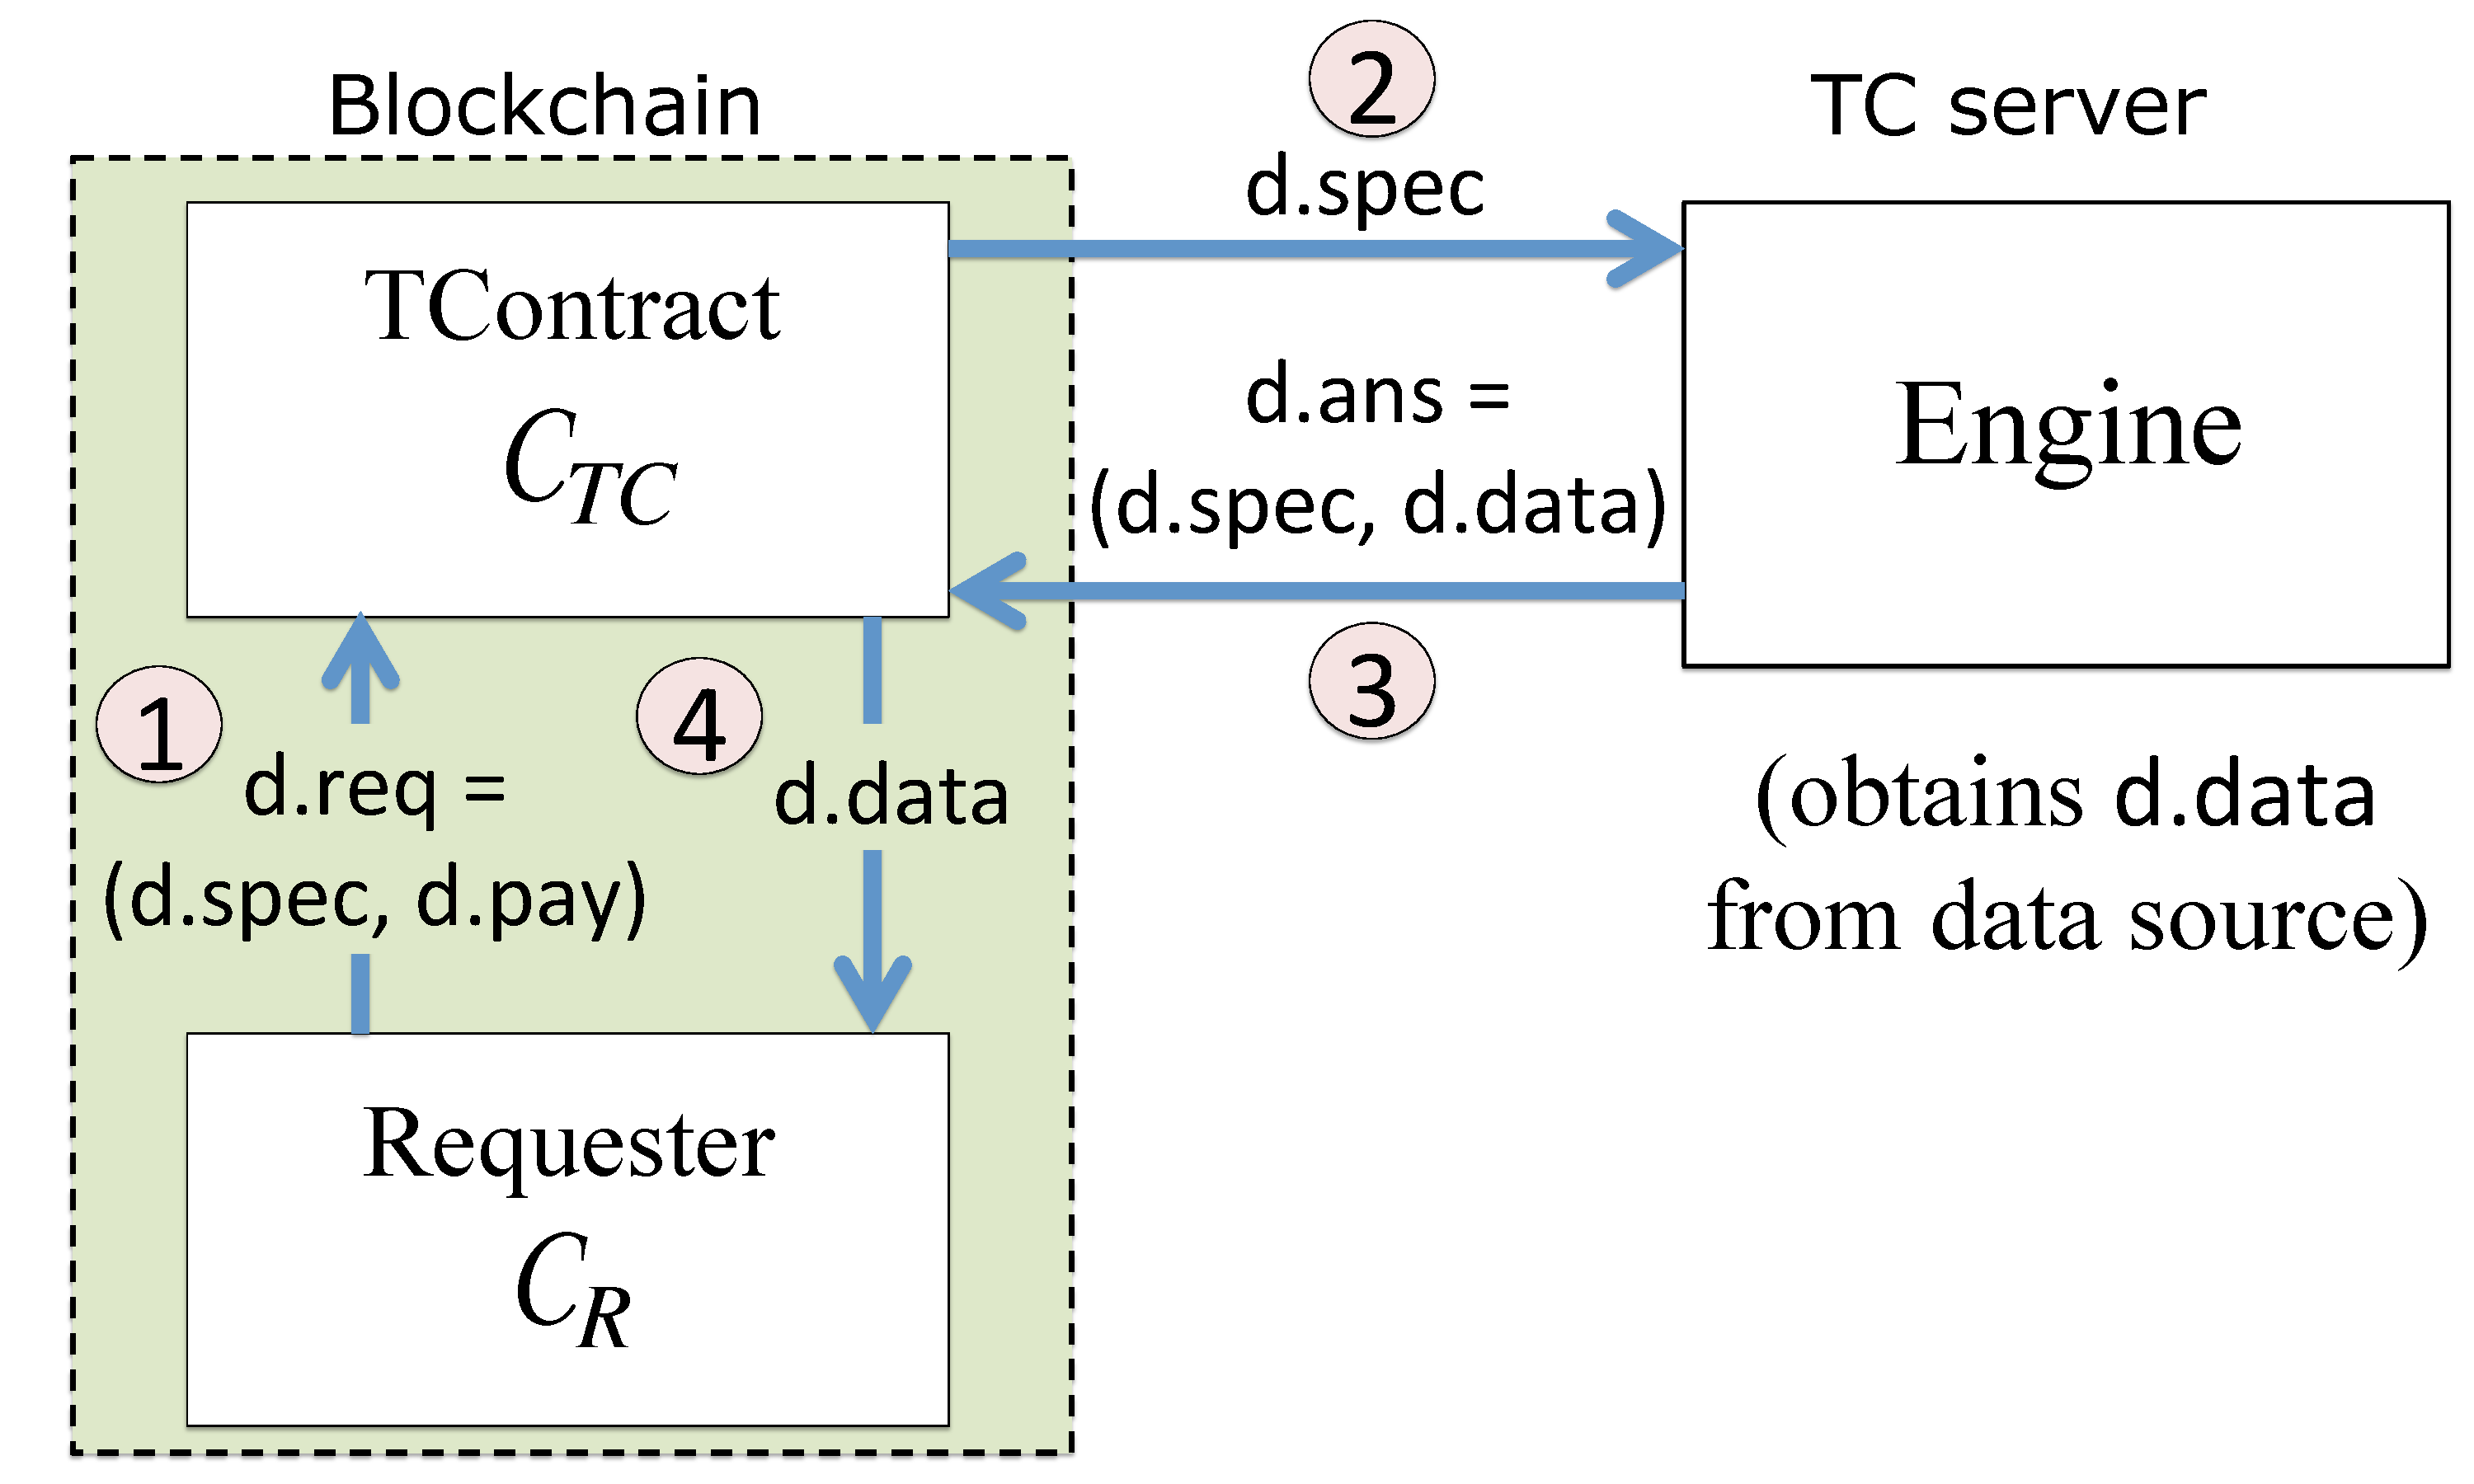
\includegraphics[width=\columnwidth]{figures/DataflowFig}
\caption{{\bf Data flows in datagram processing.}}
\label{fig:dataflow}
\end{figure}


Digital signatures are needed to authenticated messages, such as $\dgret$, entering the blockchain from an external source. We let $(\skTC, \pkTC)$ denote the private / public keypair associated with the \encname for such message authentication. For simplicity, we assume for the time that the \encname can send signed messages directly to \tcont. Later we explain how Ethereum requires a slightly different approach in which \tc sends messages via an Ethereum wallet.


\subsection{Use of SGX.}
Our protocols in \tc rely on the ability of the SGX attestation mechanism to bind an enclave process instance to a public / private key pair and for the process to high-accuracy timestamps, in absolute or wall-clock time. To simplify our presentation, we defer most details of our formal model of SGX capabilities and specification of protocols for attestation generation to the apper appendix. Instead, we first explain and present a simple abstraction of these capabilities suitable for our \tc protocol descriptions. 

Let $\enclaveprog$ represent the code for \encname, which we presume is trusted by all system participants. To avoid having to verify an EPID group signature on the blockchain, we have clients obtain SGX attestations from the \medname and verify them off-chain. As noted above, it is possible to bind an enclave process instance running \enclaveprog to a key pair $(\pkTC, \skTC)$ by including the public key pair in an attestation. We take this approach in \tc. Specifically, Since Ethereum itself 
already verifies signatures on transactions from externally owned accounts (i.e., users interact with the  Ethereum blockchain through an authenticated channel), \tc uses a trick to {\it piggyback verification of enclave signatures on top of Ethereum's already existing transaction signature verification mechanism}. Very simply, the \encname associates \pkTC with an externally owned Ethereum account \tcadd. 
This approach saves not only software engineering effort, but more importantly,  the gas that would be required for EPID signature verification.

To make this idea work fully, the public key $\pkTC$ must be hardcoded into \tcont. A client creating or relying on a contract that uses \tcont is responsible for making sure that this hardcoded $\pkTC$ has an appropriate SGX attestation before interacting with the $\tcont$  blockchain contract.  Let {\sf Verify} denote a verification algorithm for EPID signatures. Figure~\ref{fig:att_check} gives the protocol for a client to check that \tcont is backed by a valid \encname instance. This protocol does not include a mechanism for \emph{revocation} of a compromised SGX instance, an issue we discuss later in the paper.

In summary, then, we may assume in our protocol specifications that {\em all relying clients have verified an attestation for \encname and thus that \pkTC represents the public key of the associated instance.}


\paragraph{\bf Clock.}
Additionally, as noted above, trusted clock provides only relative time with  respect to a reference point, not absolute time. Thus, when initialized, the \encname is provided with the current wall-clock time by a trusted source, e.g., the \medname (under a trust-on-first-use model). The SGX attestation generated by the \encname includes the current wall-clock time, which clients may verify in real time. Thus, a client can determine the absolute clock time of \encname to within a high degree of accuracy, bounded by the round-trip time of its attestation request plus the attestation verification time--on the order of hundreds of milliseconds in a wide-area network~\cite{}.  
\ari{Let's give the attestation API a function name.} We present a formal model and protocol specification in the paper appendix.


\paragraph{\bf Notation.} We model execution in SGX in terms of a functionality $\fsgx$ operating in a stateful manner on \enclaveprog. This functionality may be be invokes through transmission of one of two messages to \enclaveprog: ``initialize'', which creates the enclave with \enclaveprog as its initial state and triggers measurement quotes and ``resume'', which initiates an execution of \enclaveprog on a fresh input. (We assume that \enclaveprog exits only when it completes processing of a given input.) We let $\fsgx[\enclaveprog, \relay]$ denote invocation of $\fsgx$ on \enclaveprog by \relay. We let $\clock()$ denote measurement of the SGX clock from within the enclave; $\clock()$ returns the current wall-clock time (in a canonical format such as seconds and fraction sections since the Unix epoch January 1, 1970 00:00 UTC).\ari{What format do we actually use?}

We abstract away the use of group signatures in EPID and simply denote the keypair associated with an SGX instance in \tc by $(\pkM, \skM)$.

\begin{figure}[htb!]
\begin{boxedminipage}{\columnwidth}
\begin{center}
{\bf User: offline attestation of SGX enclave}
\end{center}
\begin{tabular}{l}
{\bf Inputs}: $\pkM$, $\pkTC$, $\enclaveprog$, $\sigatt$ \\[5pt]
{\bf Checks:} \\
Assert $\enclaveprog$ is the expected enclave code\\
Assert $\sigsgx.{\sf Verify}(\pkM, \sigatt, (\enclaveprog, \pkTC))$ \\
Assert \tcont is correct and parametrized w/ \pkTC\\
{\it //~now okay to rely on \tcont}
\end{tabular}
\end{boxedminipage}
\label{fig:att_check}
\caption{A client checks an SGX attestation of the enclave's code and its public key $\pkTC$ and
checks that $\pkTC$ is hardcoded into \tc blockchain contract \tcont before 
making use of \tcont.
} 
\end{figure}



\subsection{A payment-free basic protocol}
For simplicity, we first specify functionalities in a payment-free version of our basic protocol, i.e., one that does not include gas or fees--specifically the message component $\dgpay$. Later, in our implementation discussion, we explain how we handle these two forms of payment, and we prove payment-related properties in the paper appendix.

\paragraph{The \tcontract}

\begin{figure}[!htb]
\begin{tabularx}{\linewidth}{|@{\hspace{3pt}}r@{\hspace{1ex}}X@{\hspace{3pt}}|}
  \hline

  \multicolumn{2}{|c|}{{\bf Town Crier blockchain contract \tcont}} \\ [1ex]
  {\bf Request:} & On recv $(\dgid, \dgform, \dgcallback)$ from some contract $\reqcont$: \\
%                 & If $(\${\sf fee} < F_{\rm min}$ or $\${\sf fee} > F_{\rm max})$ \\
%                 & \hspace*{1em} Return $\${\sf fee}$ to $\pkU$ \\
                 & Record $(\dgid, \dgform, \dgcallback)$ \\
  {\bf Deliver:} & On recv $(\dgid, \dgform, \dgm)$ from $\pkTC$: \\
		 & Let $(\dgid, \dgform, \dgcallback)$ be the most recently recorded tuple for ${\sf id}$\\
		 & Assert $\dgform = \dgform'$\\
                 & Call ${\dgcallback}({\dgm})$ \\
%                 & Send $\${\sf fee}$ ether to $\Psgx$. \\

  \hline
\end{tabularx}
\caption{
A simple, fee-free version of the Town Crier contract \tcont.
Note that communication 
with \tcont is through an authenticated channel implemented through digital signatures (which
are not explicitly expressed in our notation).
}
\label{tbl:tc-contract}
\end{figure}

\paragraph{The \encname}

\begin{figure}[!h]
\begin{boxedminipage}{\columnwidth}
\begin{center}
{\bf Town Crier's enclave program}
\end{center}
\begin{tabular}{l}
%{\bf Inputs}:  ${\sf params}$, \\[5pt]
{\bf Initialize}:  On receive ``initialize'': \\ %{\it //~called only once upfront}\\
\quad $(\pkTC, \skTC) := \Sigma.{\sf KeyGen}(1^\lambda)$\\
\quad Record $(\pkTC, \skTC)$\\
\quad Output $\pkTC$   {\it //~incl. in measurement \& attestation } 
\\[5pt]

{\bf Resume:} On receive $({\sf id}, {\sf params})$\\
\quad Parse ${\sf params} := (\weburl, \pkurl, T) $:\\
%\quad Parse ${\sf params} := (\weburl, \pkurl, T)$ \\
\quad $T_{\textrm{start}} := \clock()$\\
\quad Establish secure channel w/ $\weburl$ w/ public key $\pkurl$ \\
\quad Download the webpage at $\weburl$\\
\quad $T_{\textrm{end}}: = \clock()$\\
\quad Assert ${\sf round}(T_{\textrm{start}}) = {\sf round}(T_{\textrm{end}}) = T$\\
\quad Parse webpage and extract ${\sf data}$\\
\quad $\sigma := \Sigma.{\sf Sign}({\skTC}, ({\sf id}, {\sf params}, {\sf data}))$\\
\quad Output $(({\sf id}, {\sf params}, {\sf data}), \sigma)$
\end{tabular}
\end{boxedminipage}
\caption{
SGX enclave's code.
} 
\end{figure}

\paragraph{The \medname}

\begin{figure}[!h]
\begin{boxedminipage}{\columnwidth}
\begin{center}
{\bf Town Crier's untrusted relay $\relay$}
\end{center}
\begin{tabular}{l}
{\bf Initialize}:\\
Send ``initialize'' to $\fsgx[\enclaveprog, \relay]$\\
On receive $(\pkTC, \sigatt)$ from $\fsgx[\enclaveprog, \relay]$:\\
\quad Publish $(\pkTC, \sigatt)$\\[5pt]

{\bf  Loop forever}: \\
When \tcont receives new request $({\sf id}, \_, {\sf params})$:\\
\quad Parse ${\sf params} := (\weburl, \pkurl, T)$\\
\quad Fork: \\
\ \quad Wait till time $T$\\
\ \quad Send $(\text{``resume''}, {\sf params})$ to $\fsgx[\enclaveprog, \relay]$ \\
\ \quad On recv $(({\sf id}, {\sf params}, {\sf data}), \sigma)$ from $\fsgx[\enclaveprog, \relay]$:\\ 
\ \quad \quad  {\sf AuthSend} $({\sf id}, {\sf params}, {\sf data})$ to \tcont
\end{tabular}
\end{boxedminipage}
\caption{Town Crier untrusted relay. For simplicity, here we assume that there is only 
a single enclave program. When multiple data feed sources 
are supported, 
we need multiple enclaves that instantiate different parsers for different sites.
In this case, the Town Crier relay also initialize all enclave instances
and route the request to the correct enclave instance.}
\end{figure}




